\documentclass[a4paper]{article} 
\addtolength{\hoffset}{-2.25cm}
\addtolength{\textwidth}{4.5cm}
\addtolength{\voffset}{-3.25cm}
\addtolength{\textheight}{5cm}
\setlength{\parskip}{0pt}
\setlength{\parindent}{0in}

%----------------------------------------------------------------------------------------
%	PACKAGES AND OTHER DOCUMENT CONFIGURATIONS
%----------------------------------------------------------------------------------------

\usepackage[italicdiff]{physics}
%\usepackage{derivative}
\usepackage{tasks}
\usepackage{blindtext} % Package to generate dummy text
\usepackage{charter} % Use the Charter font
\usepackage[utf8]{inputenc} % Use UTF-8 encoding
\usepackage{microtype} % Slightly tweak font spacing for aesthetics
\usepackage[T1]{fontenc}
\usepackage{polski}
\usepackage{enumerate}
\usepackage[utf8]{inputenc}
\usepackage[english, ngerman]{babel} % Language hyphenation and typographical rules
\usepackage{amsthm, amsmath, amssymb} % Mathematical typesetting
\usepackage{float} % Improved interface for floating objects
\usepackage[final, colorlinks = true, 
            linkcolor = black, 
            citecolor = black]{hyperref} % For hyperlinks in the PDF
\usepackage{graphicx, multicol} % Enhanced support for graphics
\usepackage{xcolor} % Driver-independent color extensions
\usepackage{marvosym, wasysym} % More symbols
\usepackage{rotating} % Rotation tools
\usepackage{censor} % Facilities for controlling restricted text
\usepackage{listings, style/lstlisting} % Environment for non-formatted code, !uses style file!
\usepackage{pseudocode} % Environment for specifying algorithms in a natural way
\usepackage{style/avm} % Environment for f-structures, !uses style file!
\usepackage{booktabs} % Enhances quality of tables
\usepackage{tikz-qtree} % Easy tree drawing tool
\tikzset{every tree node/.style={align=center,anchor=north},
         level distance=2cm} % Configuration for q-trees
\usepackage{style/btree} % Configuration for b-trees and b+-trees, !uses style file!
\usepackage[backend=biber,style=numeric,
            sorting=nyt]{biblatex} % Complete reimplementation of bibliographic facilities
\addbibresource{ecl.bib}
\usepackage{csquotes} % Context sensitive quotation facilities
\usepackage[yyyymmdd]{datetime} % Uses YEAR-MONTH-DAY format for dates
\renewcommand{\dateseparator}{-} % Sets dateseparator to '-'
\usepackage{fancyhdr} % Headers and footers
\pagestyle{fancy} % All pages have headers and footers
\fancyhead{}\renewcommand{\headrulewidth}{0pt} % Blank out the default header
\fancyfoot[L]{} % Custom footer text
\fancyfoot[C]{} % Custom footer text
\fancyfoot[R]{\thepage} % Custom footer text
\newcommand{\note}[1]{\marginpar{\scriptsize \textcolor{red}{#1}}} %
\graphicspath{ {./images/} }

%----------------------------------------------------------------------------------------

\begin{document}

%-------------------------------
%	TITLE SECTION
%-------------------------------

\fancyhead[C]{}
\hrule \medskip % Upper rule
\begin{minipage}{0.295\textwidth} 
\raggedright
\footnotesize
Antoni Dąbrowski \hfill\\   
Nr. indeksu 317214\hfill\\
Mail: 317214@uwr.edu.pl
\end{minipage}
\begin{minipage}{0.4\textwidth} 
\centering 
\large 
Statystyka\\ 
\normalsize 
Laboratorium - lista III\\ 
\end{minipage}
\begin{minipage}{0.295\textwidth} 
\raggedleft
\today\hfill\\
\end{minipage}
\medskip\hrule 
\bigskip

%-------------------------------
%	CONTENTS
%-------------------------------


\section{Zadanie pierwsze}
Podaj przedział ufności dla średniej w modelu normalnym o znanej wariancji na poziomie ufności $1-\alpha$. Uzasadnij jego postać.


\subsection{Rozwiązanie}
$\sigma^2$ - znane, $\mu$ - szukane

$$\bar{X}_n\sim N(\mu,\frac{\sigma^2}{n})$$

Dla rozkładu normalnego:
$$\frac{1}{\sigma\sqrt{n}}\sum_{i=0}^n(X_i-\mu)\sim N(0,1)$$

Dla dowolnego innego (z centralnego twierdzenia granicznego):
$$\frac{1}{\sigma\sqrt{n}}\sum_{i=0}^n(X_i-\mu)\rightarrow N(0,1)$$

Zatem:
$$P(-z_{\alpha/2}\leq\frac{1}{\sigma\sqrt{n}}\sum_{i=0}^n(X_i-\mu)\leq z_{\alpha/2})=1-\alpha$$

Przekształcając wychodzi, że przedział ufności dla $mu$ to:
$$(\bar{X}_n-z_{\alpha/2}\frac{\sigma}{\sqrt{n}},\bar{X}_n+z_{\alpha/2}\frac{\sigma}{\sqrt{n}})$$

Gdzie $z_{\alpha/2}$ to odwrotna dystybuanta rozkładu normalnego:
$$z_{\alpha/2}=\Phi^{-1}(\alpha/2)$$


\section{Zadanie drugie}
Wygeneruj $n=50$ obserwacji z rozkładu
\begin{enumerate}[a.]
	\item normalnego z parametrem przesunięcia $\mu$ i skali $\sigma$
	\item logistycznego z parametrami przesunięcia $\mu$ i skali $\sigma$
	\item Cauch'ego z parametrami przesunięcia $\mu$ i skali $\sigma$
	\item wykładniczego z parametrem przesunięcia $\lambda$
	\item chi-kwadrat z $\nu$ stopniami swobody
\end{enumerate}
Na tej podstawie wyznacz przedziały ufności dla średniej z zadania 1 na poziomie ufności 0.95 oraz jego długość. Doświadczenie powtórz 10 000 razy. Oszacuj prawdopodobieństwo pokrycia nieznanej średniej przez przedział ufności oraz jego dzługość. Przedyskutuj uzyskane wyniki.


\subsection{Rozwiązanie}
Poniższe wykresy przedstawiają $1\%$ spośród 10000 losowań 50-elementowych próbek. Zielona linia określa prawdziwą wartość estymowanego parametru. Pionowe słupki to przedziały ufności wokół estymatu punktowego, czerwone słupki oznaczają przedziały nie zawierające prawdziwej wartości. Pod wykresem podaję parametry rozkładu, liczbę błędnie określonych przedziałów ufności (takich, które nie pokrywają wartości rzeczywistej). Dalej podaję przedział ufności i jego długość wyznaczone jako mediana spośród wszystkich prób.

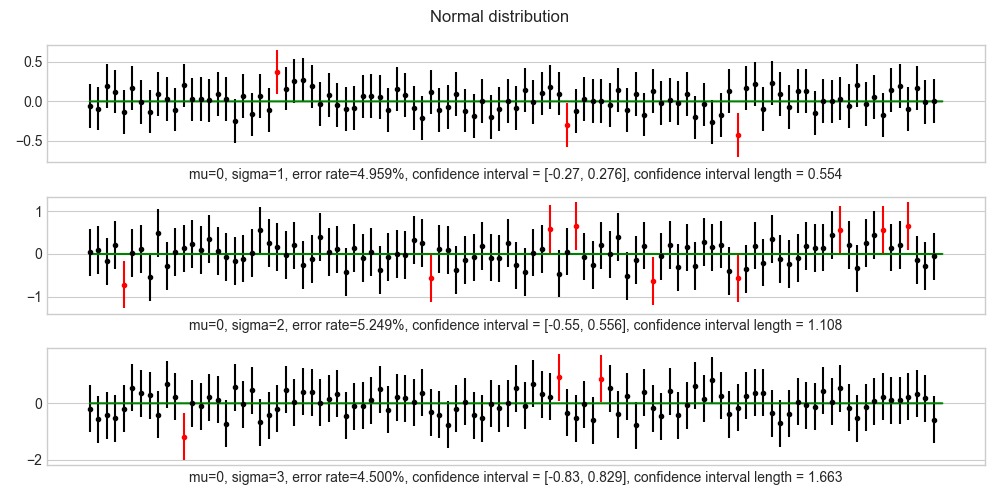
\includegraphics[scale=0.65]{Z2a}

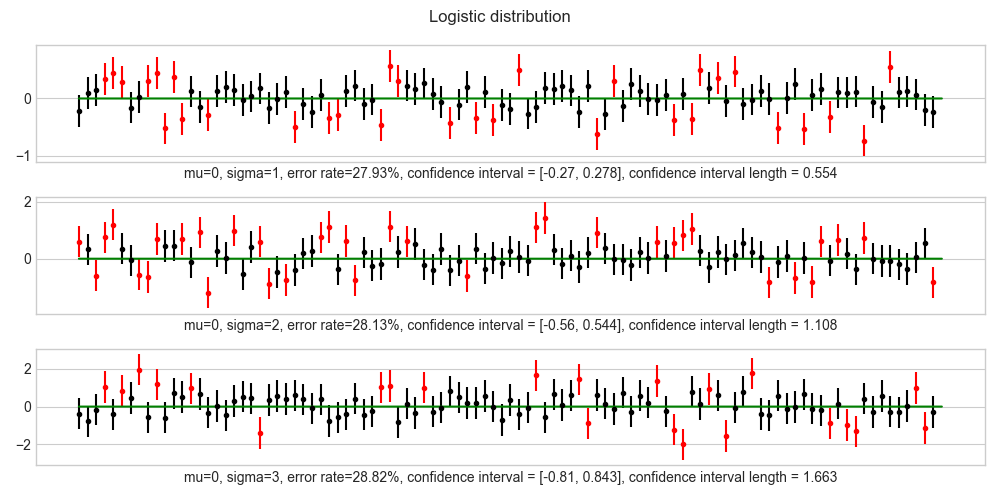
\includegraphics[scale=0.65]{Z2b}

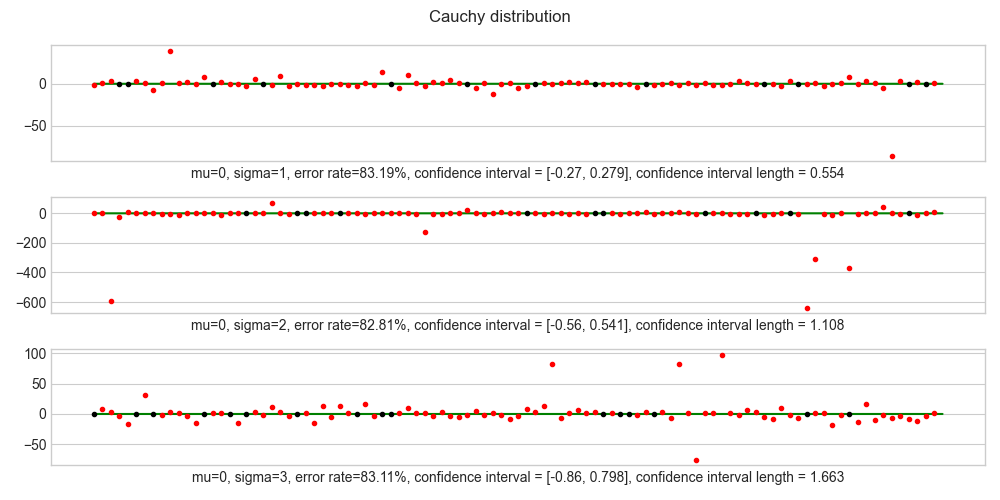
\includegraphics[scale=0.65]{Z2c}

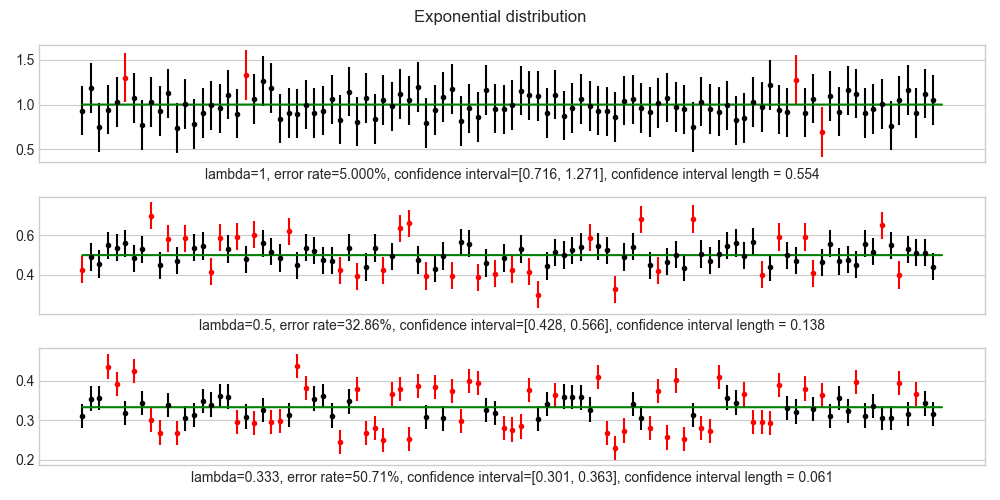
\includegraphics[scale=0.65]{Z2d}

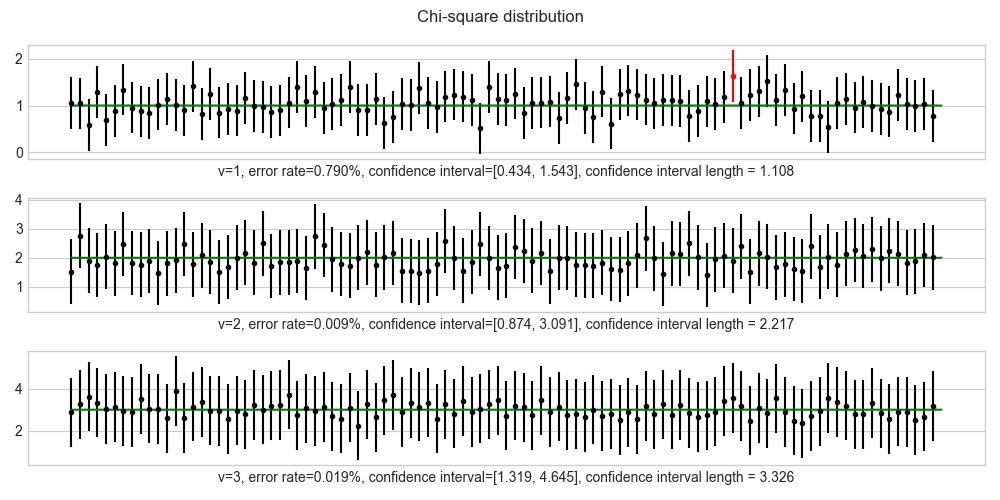
\includegraphics[scale=0.65]{Z2e}

\textbf{Obserwacje:}

Teoria z zadania pierwszego sprawdza się w praktyce. Przedział ufności dla rozkładu normalnego i poziomu ufności $95\%$ faktycznie w takim stopniu pokrywa dokładną wartość. Nie jest tak jednak dla pozostałych rozkładów. Przyczynę tego spodziewam się znaleźć w nie dość dużej próbie, gdzyż teoria mówi, że asymptotycznie powinniśmy otrzymać dobry przedział.

\section{Zadanie trzecie}
Podaj przedział ufności dla średniej w modelu normalnym o nieznanej wariancji na poziomie ufności $1-\alpha$. Uzasadnij jego postać.

\subsection{Rozwiązanie}
\textbf{Twierdzenie 1.}
Niech $Z$ będzie zmienną losową o rozkładzie normalnym, $U$ będzie zmienną losową o rozkładzie $\chi^2$ z $\nu$ stopniami swobody, niech zmienne $U$ i $Z$ będą niezależne, wtedy nowa zmienna:
$$T=\frac{Z}{\sqrt{U/\nu}}$$
ma rozkład t Studenta z $\nu$ stopniami swobody.

\textbf{Kontynuacja rozwiązania:}



$\sigma^2$ - nie znane, $\mu$ - szukane

$$\bar{X}_n\sim N(\mu,\frac{\sigma^2}{n})\land\sum_{i=1}^n(X_i-\bar{X}_n)^2\sim\chi_{n-1}^2\implies\frac{\bar{X}_n-\mu}{\sqrt{\sum_{i=1}^n(X_i-\bar{X}_n)^2/(n-1)}}\sim t_{n-1}$$

$$P(-t_{\alpha/2}\leq\frac{\bar{X}_n-\mu}{\sqrt{\sum_{i=1}^n(X_i-\bar{X}_n)^2/(n-1)}}\leq t_{\alpha/2})=1-\alpha$$

Stąd przedział ufności dla $mu$ to:
$$(\bar{X}_n-t_{\alpha/2}\frac{\sqrt{\sum_{i=1}^n(X_i-\bar{X}_n)^2}}{\sqrt{n-1}},\bar{X}_n+t_{\alpha/2}\frac{\sqrt{\sum_{i=1}^n(X_i-\bar{X}_n)^2}}{\sqrt{n-1}})$$

Gdzie $t_{\alpha/2}$ to odwrotna dystybuanta rozkładu t Studenta:
$$t_{\alpha/2}=\Phi^{-1}(\alpha/2)$$

Dla dużej próby w zasadzie można by użyć metody z zadania pierwszego, ponieważ rozkład t Studenta zbiega do rozkładu normalnego wraz ze wzrostem stopnia swobody.


\section{Zadanie czwarte}
Powtórz eksperyment numeryczny z zadania 2. Na jego podstawie oszacuj prawdopodobieństwo pokrycia nieznanej średniej przez przedział ufności z zadania 3 na poziomie ufności 0.95 oraz jego długość. Przedyskutuj uzyskane rezultaty.


\subsection{Rozwiązanie}

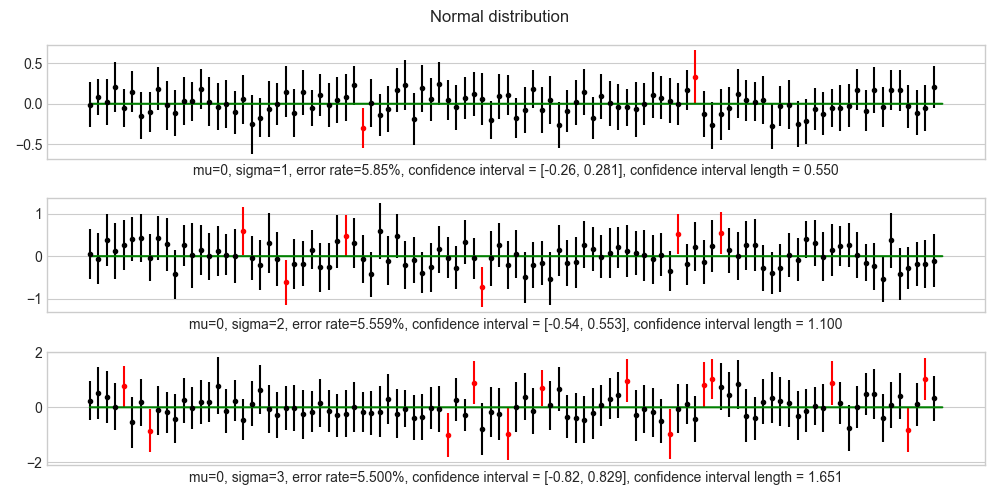
\includegraphics[scale=0.65]{Z4a}

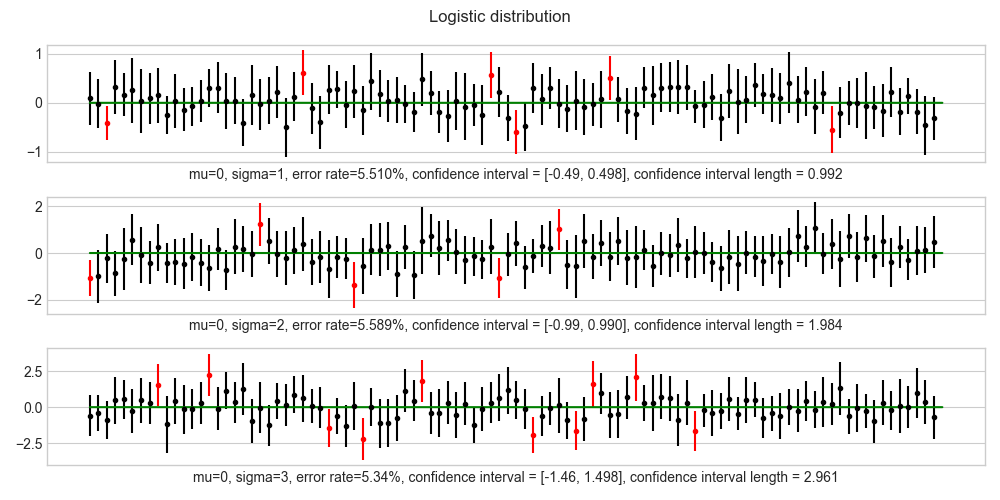
\includegraphics[scale=0.65]{Z4b}

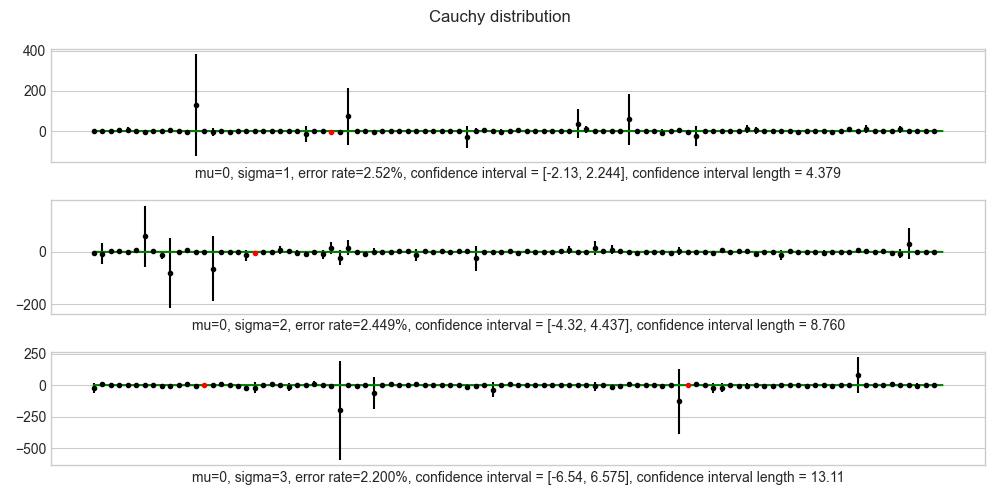
\includegraphics[scale=0.65]{Z4c}

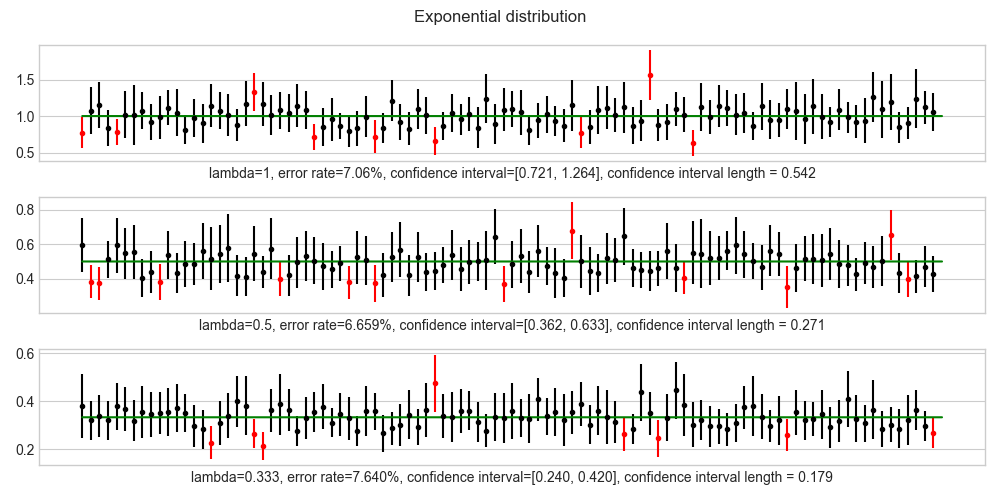
\includegraphics[scale=0.65]{Z4d}

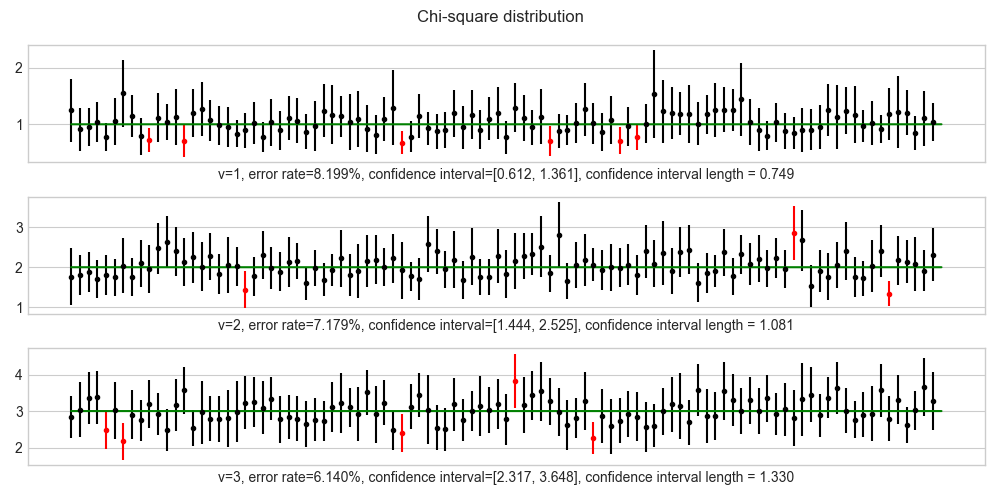
\includegraphics[scale=0.65]{Z4e}

W przypadku rozkładu normalnego otrzymałem podobne rezultaty do tych z zadania drugiego. Jednak w przypadku pozostałych rozkładów znalezione przedziały ufności były znacznie dłuższe. Mniejsza niepewność w zadaniu drugim prawdopodobnie wynika z dodatkowej wiedzy jaką jest wartość dokładna wariancji.

\section{Zadanie piąte}
Podaj przedział ufności dla wariancji w modelu normalnym o znanej średniej na poziomie ufności $1-\alpha$. Uzasadnij jego poprawność.

\subsection{Rozwiązanie}
$\sigma^2$ - szukane, $\mu$ - znane

Można rozwiązać to zadanie analogicznie do kolejnego, gdzie średnia jest nieznana. Jednak skoro ją znam, to intuicyjnie wydaje się, że można uzyskać lepsze wyniki używając jej do wyznaczenia wariancji próbkowej (zamiast średniej próbkowej).


\section{Zadanie szóste}
Powtórz eksperyment numeryczny z zadania 2. Na jego podstawie oszacuj prawdopodobieństwo pokrycia nieznanej wariancji przez przedział ufności z zadania 5 na poziomie ufności 0.95 oraz jego długość. Przedyskutuj uzyskane rezultaty.

\subsection{Rozwiązanie}

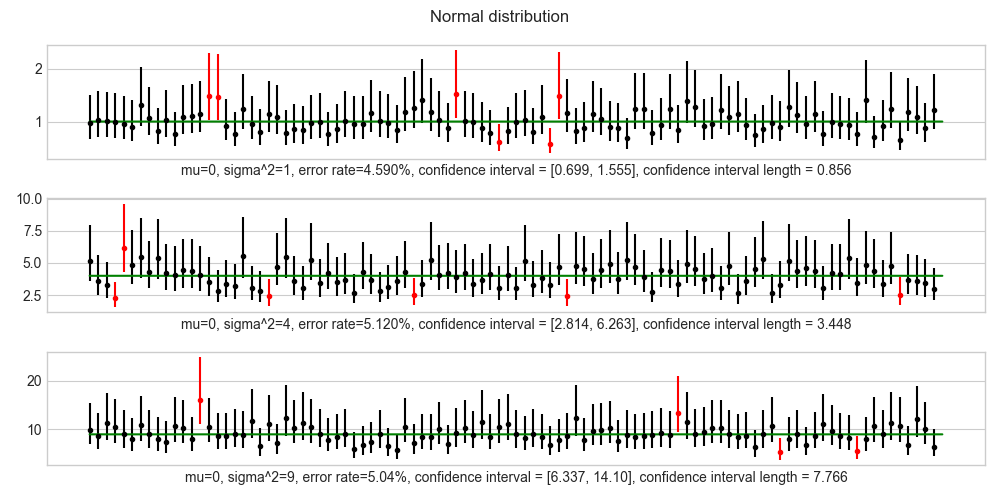
\includegraphics[scale=0.65]{Z6a}

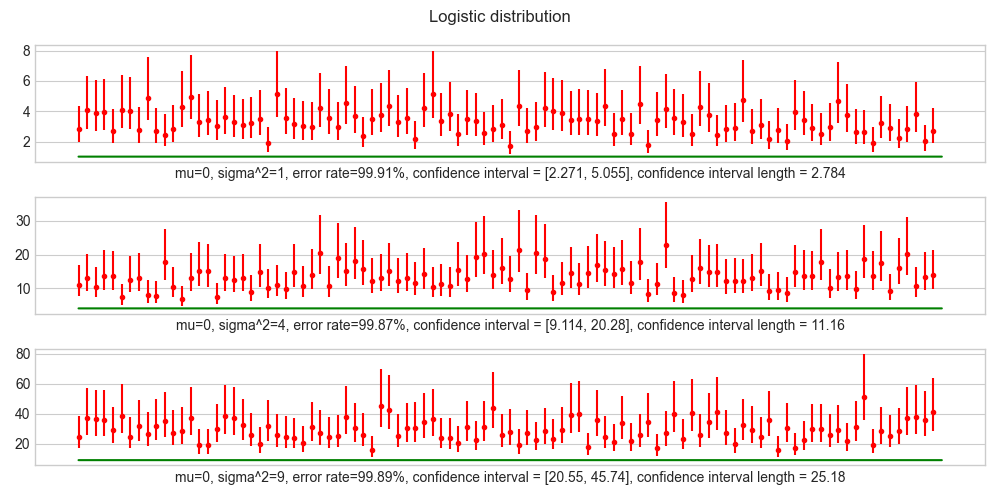
\includegraphics[scale=0.65]{Z6b}

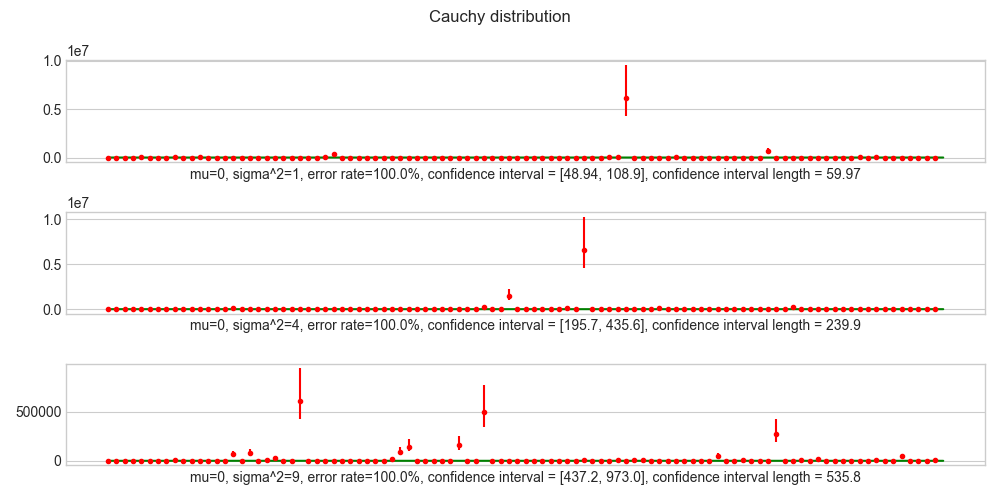
\includegraphics[scale=0.65]{Z6c}

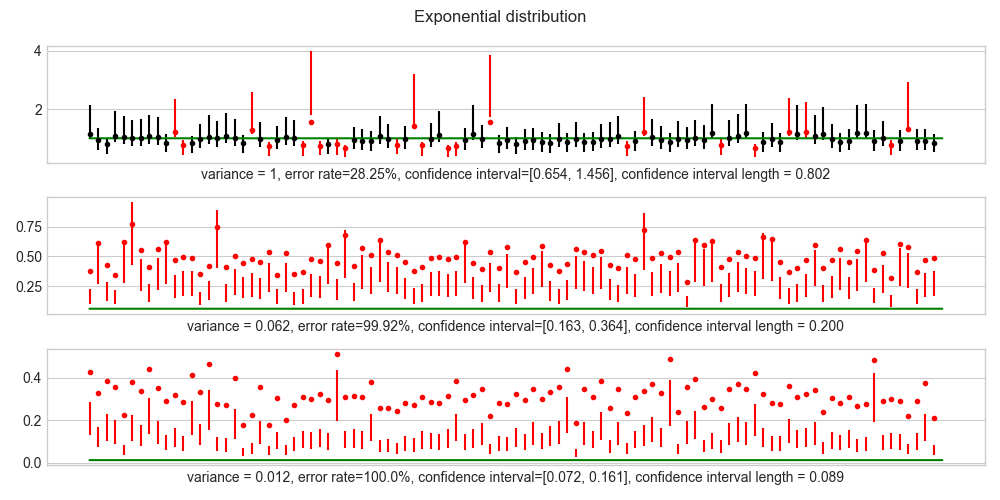
\includegraphics[scale=0.65]{Z6d}

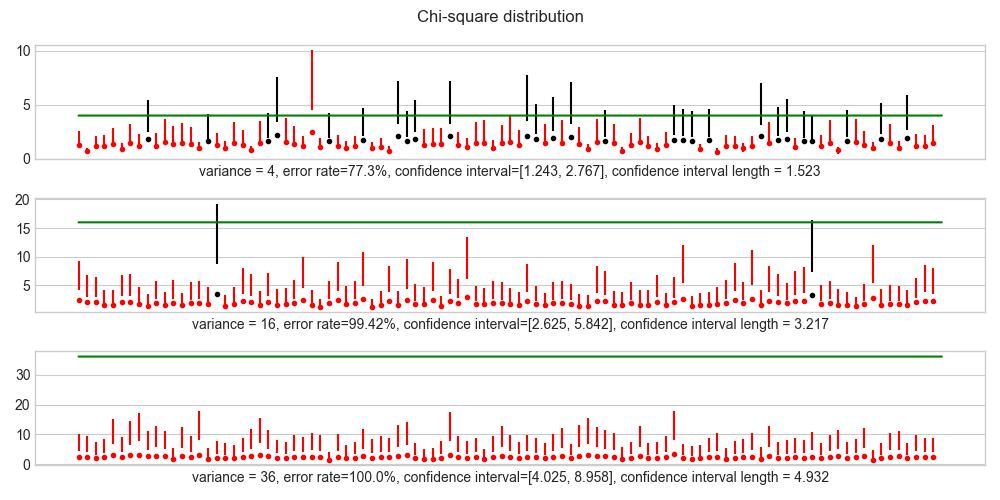
\includegraphics[scale=0.65]{Z6e}

Teoria z poprzedniego zadania dobrze sprawdza się w przypadku rozważanego rozkładu normalnego, jednak nie ma żadnej pewności, że będzie ona działać dla dowolnego innego rozkładu, co widać na powyższych wykresach.


\section{Zadanie siódme}
Podaj przedział ufności dla wariancji w modelu normalnym o nieznanej średniej na poziomie ufności $1-\alpha$. Uzasadnij jego poprawność.

\subsection{Rozwiązanie}
$\sigma^2$ - szukane, $\mu$ - nie znane

Niech $s^2=\frac{1}{n-1}\sum_{i=1}^n(X_i-\bar{X}_n)^2$ oznacza variancję próbki. Wtedy $\frac{(n-1)s^2}{\sigma^2}\sim\chi^2$ z $n-1$ stopniami swobody. Stąd:

$$P(\chi^2_{\alpha/2}\leq\frac{(n-1)s^2}{\sigma^2}\leq\chi^2_{1-\alpha/2})=1-\alpha$$
gdzie $\chi^2_{1-\alpha/2}$ jest kwantylem rzędu ${1-\alpha/2}$ rozkładu $\chi^2$ o $n-1$ stopniach swobody, a $\chi^2_{\alpha/2}$ jest odpowiednio kwantylem rzędu $\alpha/2$. Ponieważ funkcja gęstości rozkładu $\chi^2$ nie jest symetryczna również przedział ufności nie będzie symetryczny. Przekształcając otrzymamy szukany przedział:
$$P(\frac{\chi^2_{\alpha/2}}{(n-1)s^2}\leq\frac{1}{\sigma^2}\leq\frac{\chi^2_{1-\alpha/2}}{(n-1)s^2})=1-\alpha$$
$$P(\frac{(n-1)s^2}{\chi^2_{\alpha/2}}\geq\sigma^2\geq\frac{(n-1)s^2}{\chi^2_{1-\alpha/2}})=1-\alpha$$
$$P(\frac{(n-1)s^2}{\chi^2_{1-\alpha/2}}\leq\sigma^2\leq\frac{(n-1)s^2}{\chi^2_{\alpha/2}})=1-\alpha$$

Stąd przedział ufności dla $\sigma^2$ to:
$$(\frac{(n-1)s^2}{\chi^2_{1-\alpha/2}},\frac{(n-1)s^2}{\chi^2_{\alpha/2}})$$

\section{Zadanie ósme}

\subsection{Rozwiązanie}

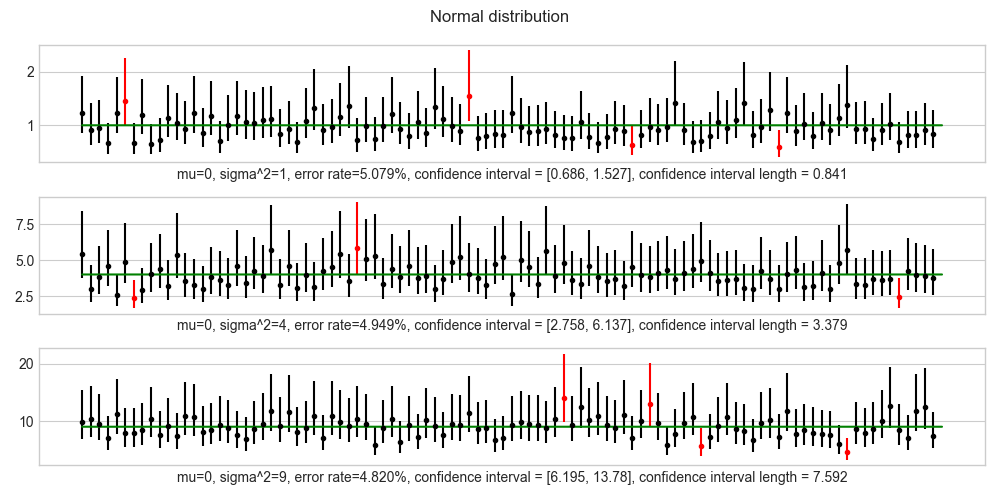
\includegraphics[scale=0.65]{Z8a}

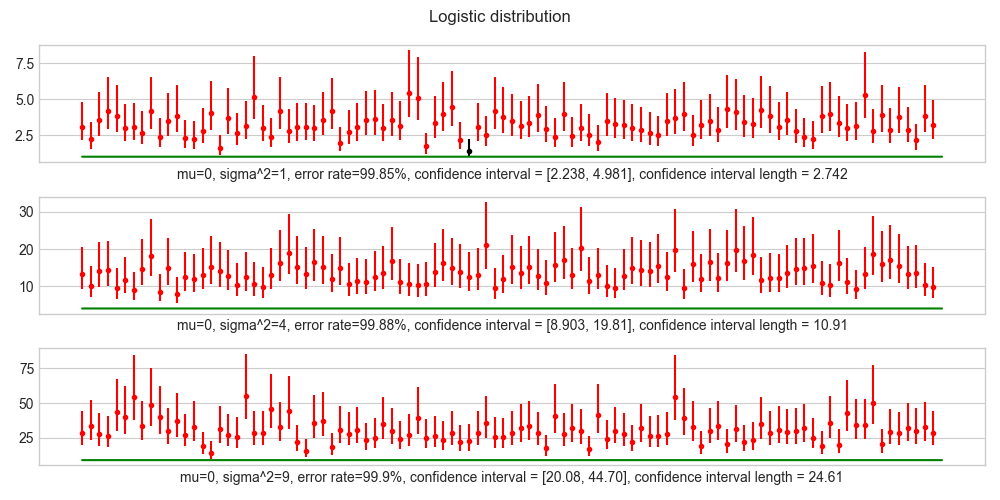
\includegraphics[scale=0.65]{Z8b}

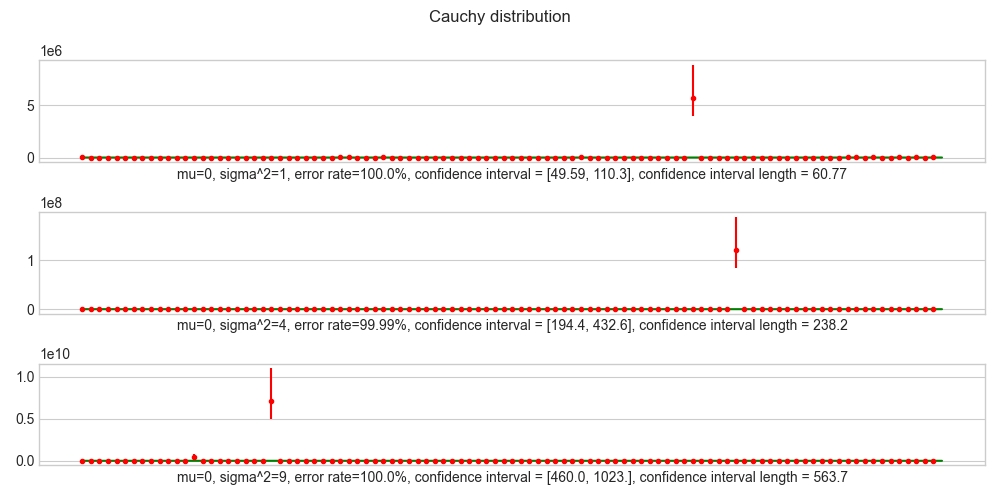
\includegraphics[scale=0.65]{Z8c}

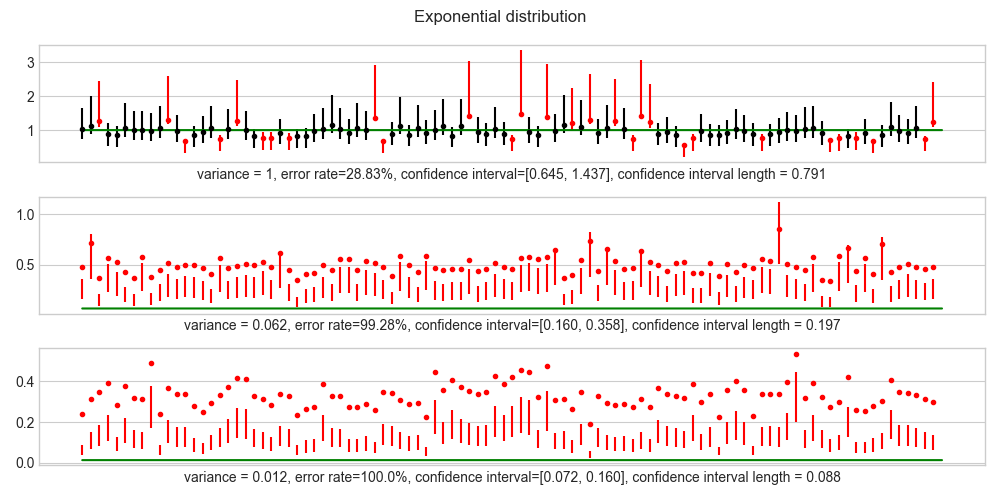
\includegraphics[scale=0.65]{Z8d}

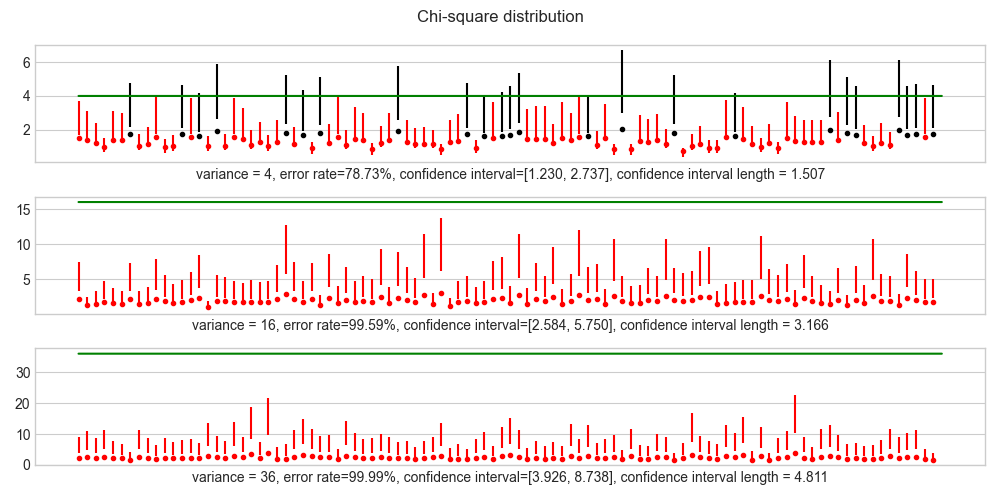
\includegraphics[scale=0.65]{Z8e}

Brak informacji o średniej nie wpłyną znacząco na rezultaty.

\section{Zadanie dziewiąte}
Podaj asymptotyczny przedział ufności dla proporcji na poziomie ufności $1-\alpha$. Uzasadnij jego postać.

\subsection{Rozwiązanie}
Niech $X$ będzie zmienną losową o rozkładzie $B(n,p)$, chcemy na podstawie realizacji tej zmiennej oszacować wartość $p$. Niech $X_1,...,X_n$ będzie próbą losową z określonego rozkładu, wtedy za estymat punktowy $p$, weźmiemy $\hat{p}=\bar{X}$. Z centralnego twierdzenia granicznego wiadomo, że $\hat{p}$ asymptotycznie ma rozkład $N(p,p(1-p)/n)$. Ponieważ $\hat{p}$ asymptotycznie zbiega do $p$, a $\hat{p}(1-\hat{p})$ zbiega do $p(1-p)$ to:
$$P(-z_{\alpha/2}\leq\frac{p-\hat{p}}{\sqrt{\hat{p}(1-\hat{p})/n}}\leq z_{\alpha/2})=1-\alpha$$
$$P(\hat{p}-z_{\alpha/2}\sqrt{\hat{p}(1-\hat{p})/n}\leq p\leq\hat{p}+z_{\alpha/2}\sqrt{\hat{p}(1-\hat{p})/n})=1-\alpha$$

Stąd asymptotyczny przedział ufności dla $p$ to:
$$(\hat{p}-z_{\alpha/2}\sqrt{\hat{p}(1-\hat{p})/n},\hat{p}+z_{\alpha/2}\sqrt{\hat{p}(1-\hat{p})/n})$$

Gdzie $z_{\alpha/2}$ to odwrotna dystybuanta rozkładu normalnego:
$$z_{\alpha/2}=\Phi^{-1}(\alpha/2)$$

\section{Zadanie dziesiąte}
Powtórz eksperyment numeryczny z zadania 2, podpunkty: a, b, c. Na jego podstawie oszacuj prawdopodobieństwo pokrycia nieznanej proporcji dodatnich obserwacji przez przedział ufności z zadania 9 na poziomie ufności 0.95 oraz jego długość. Przedyskutuj uzyskane rezultaty.

\subsection{Rozwiązanie}

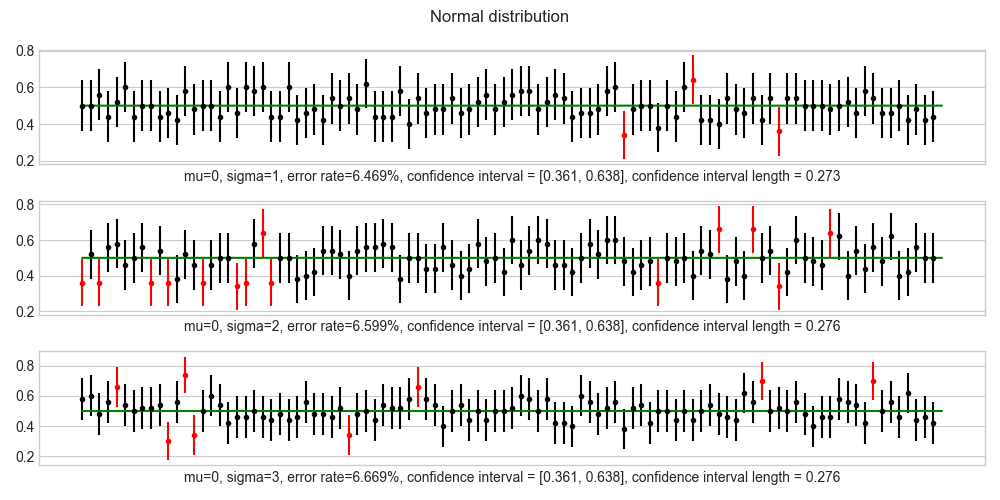
\includegraphics[scale=0.65]{Z10a}

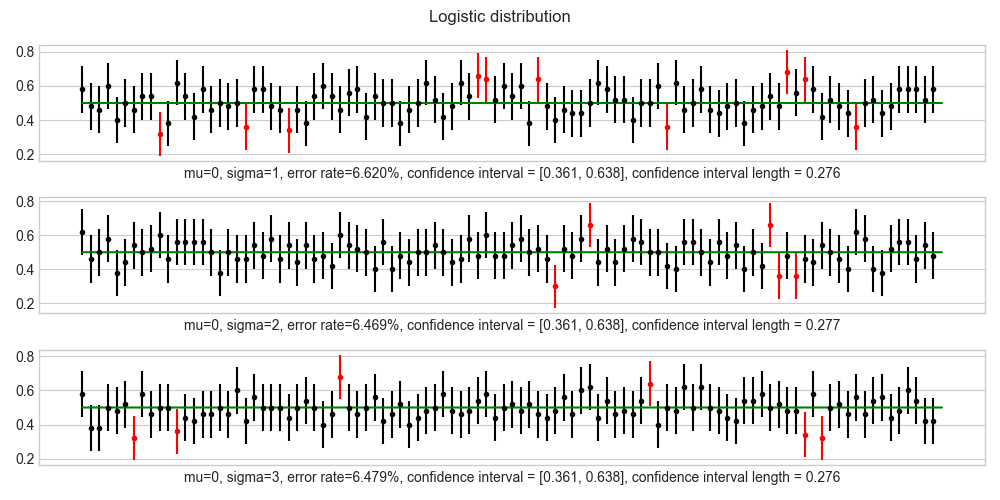
\includegraphics[scale=0.65]{Z10b}

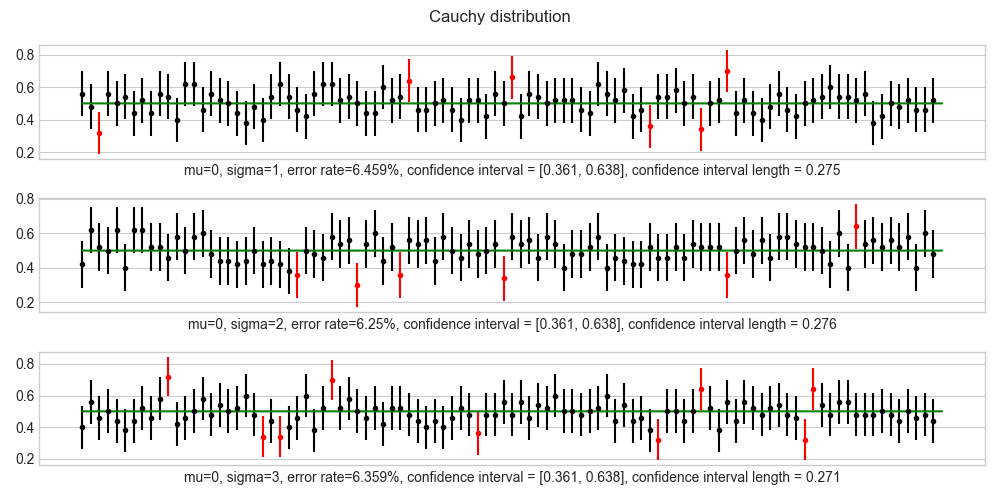
\includegraphics[scale=0.65]{Z10c}

Powyższe wyniki potwierdzają prawdziwość teori dyskutowanej w poprzednim zadaniu. Przedziały ufności zdają się pokrywać z zadaną pewnością wartość dokładną.

\section{Zadanie jedenaste}
Powtórz eksperyment numeryczny z zadań 2, 4, 6, 8, 10, dla $n=20$ i $n=100$. Przedyskutuj uzyskane rezultaty w nawiązaniu do wcześniejszych wyników.

\subsection{Rozwiązanie}

Dla przejrzystości nie będę zamieszczał wszystkich wykresów, opiszę jedynie główne obserwacje.
\begin{itemize}
\item Wraz ze wzrostem liczby obserwacji długość przedziału ufności maleje.
\item Błędne przedziały funości w zadaniu szóstym i ósmym nie są wynikiem zbyt małej próby
\item Wartości error rate z zadania 10 faktycznie zbiegają do $5\%$
\end{itemize}

\end{document}
